\newpage

\section{Partial Redundancy Elimination}
Partial redundancy elimination (PRE) is a global optimization introduced by Morel and Renvoise\cite{morel1979global}. It
combines and extends two other techniques: common subexpression elimination and loop-invariant code motion. 

An expression is partially redundant at point p if it
is redundant along some, but not all, paths that reach
p. PRE converts partially-redundant expressions into
redundant expressions. The basic idea is simple. First,
it uses data-flow analysis to discover where expressions
are partially redundant. Next, it solves a data-flow
problem that shows where inserting copies of a computation would convert a partial redundancy into a full
redundancy. Finally, it inserts the appropriate code and
deletes the redundant copy of the expression.

A key feature of PRE is that it never lengthens an
execution path. To see this more clearly, consider the
example shown in Figure \ref{fig:p82}. In the fragment on the left, the second
computation of \texttt{x + y} is partially redundant; it is only
available along one path from the if. Inserting an evaluation of 
\texttt{x + y} on the other path makes the computation
redundant and allows it to be eliminated, as shown in
the right-hand fragment. Note that the left path stays
the same length while the right path has been shortened.


\begin{figure}[H]
    \centering
     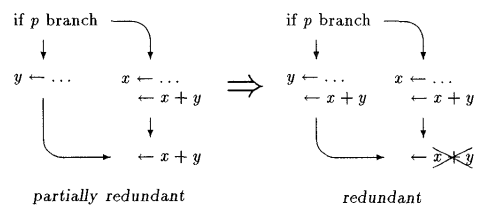
\includegraphics[width=0.5\textwidth]{p82.png}
         \caption{}
         \label{fig:p82}
\end{figure}


Loop-invariant expressions are also partially redundant,
as shown in Figure \ref{fig:p83}. On the left, \texttt{x + y} is
partially redundant since it is available from one predecessor 
(along the back edge of the loop), but not the
other. Inserting an evaluation of \texttt{x + y} before the loop
allows it to be eliminated from the loop body.


\begin{figure}[H]
    \centering
     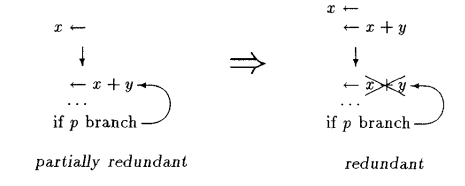
\includegraphics[width=0.5\textwidth]{p83.png}
         \caption{}
         \label{fig:p83}
\end{figure}


\subsection{Finding Partially Available Expressions}

For every expression, we can do a dataflow analysis.

\begin{center}
    \begin{tabular}{|c|c|}
   \hline Direction & Forward\\
   \hline Meet operator & \( \cup \)\\
   \hline Lattice & \( \{ 0,1 \} \)\\
   \hline Top(T) & \( 0 \)\\
   \hline Bottom &  \( 1 \)\\
   \hline Boundary condition for entry node & \( 0 \) \\  
   \hline Initialization for internal nodes & \(\mathrm{T}\) \\
   \hline Finited escending chain? &\checkmark  \\
   \hline Transferfunction  &  \( PAVOUT[i] =  (PAVIN[i] - KILL[i]) \cup AVLOC[i]\)\\
   \hline Monotone\&Distributive?  & \checkmark \\
   \hline AVLOC  & {Expression is {\color{blue}locally available (AVLOC)} if downwards exposed.  }\\
   \hline KILL & Expression is {\color{blue}killed ( KILL)} if any assignments to operands. \\
   \hline
   \end{tabular}  
   \end{center}


   \begin{figure}[H]
    \centering
     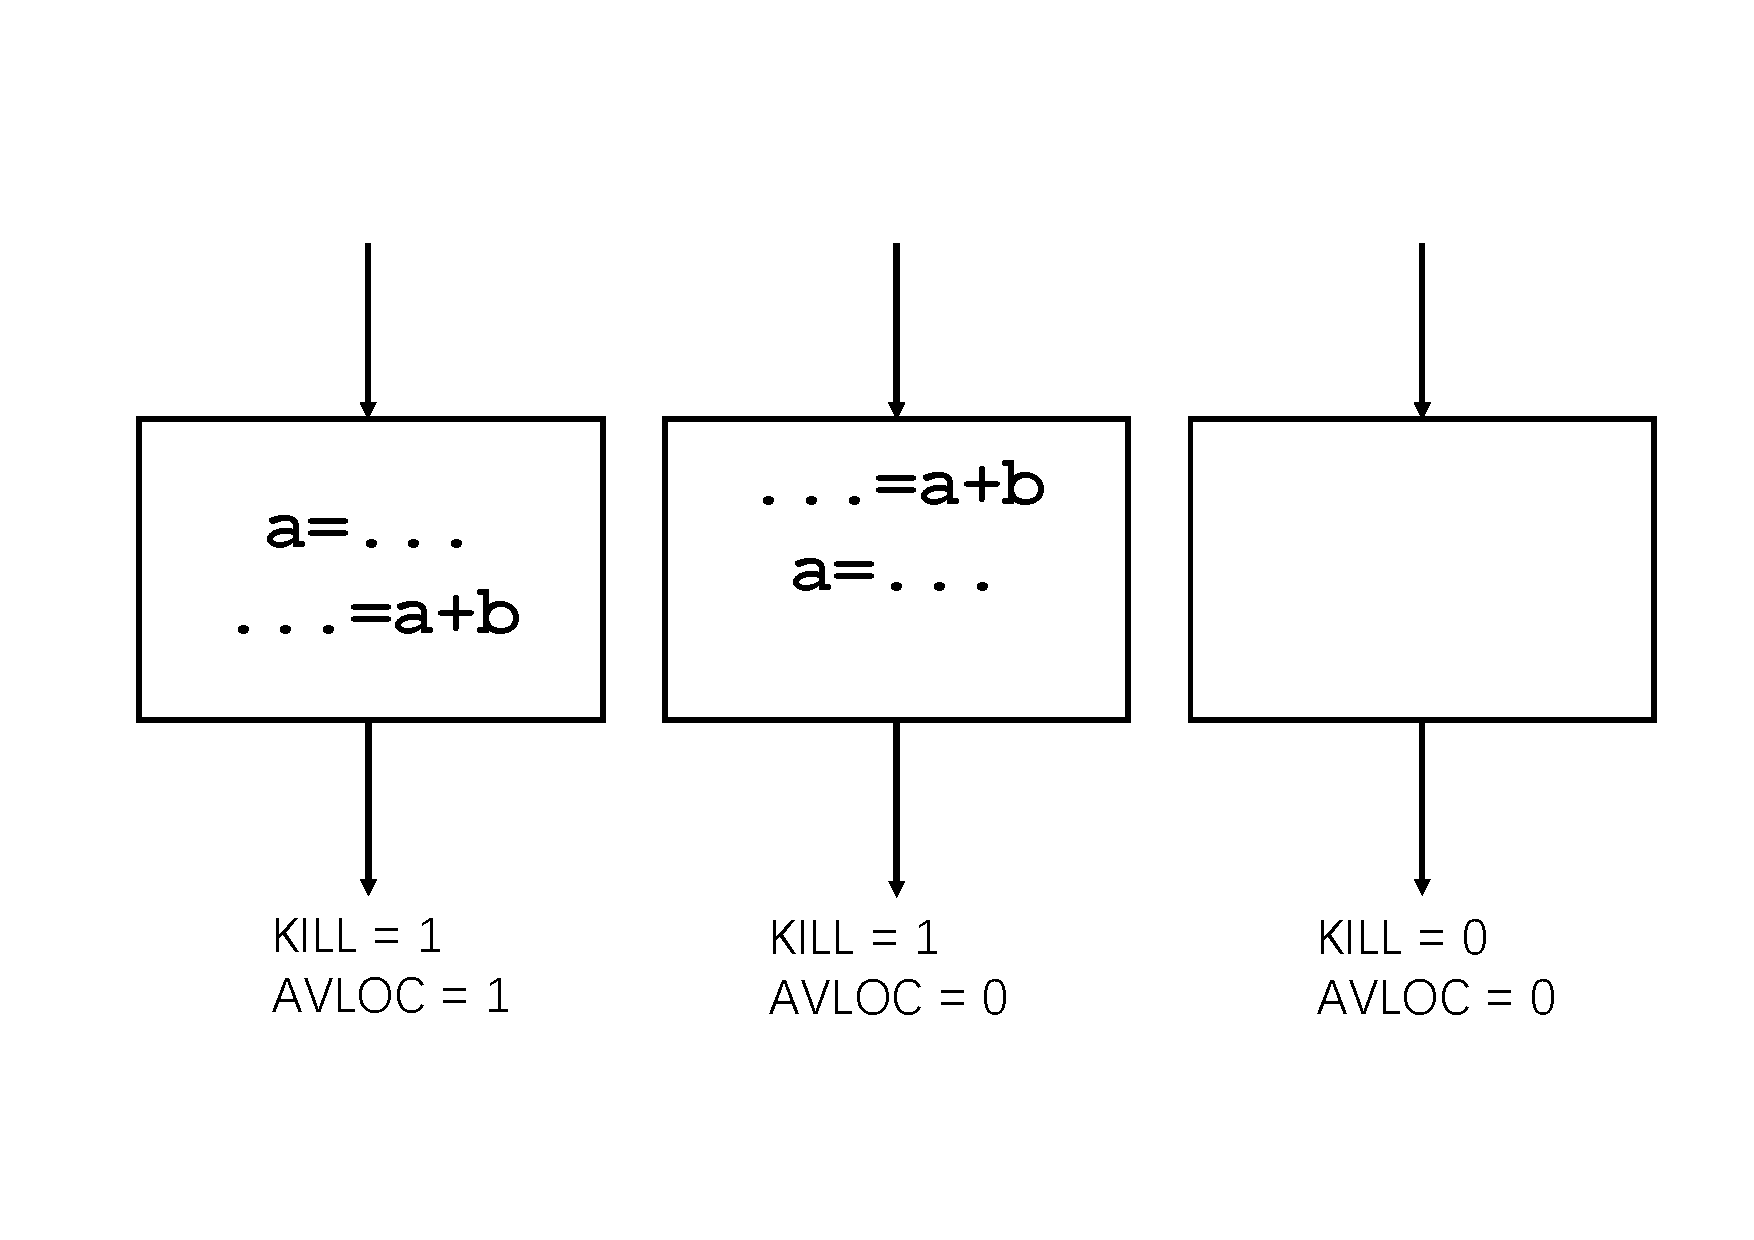
\includegraphics[width=0.8\textwidth]{p84.pdf}
         \caption{For \texttt{a+b}, the result of  Partially Available Expressions's transfer function within a basic block.}
         \label{fig:p84}
\end{figure}



\begin{figure}[H]
    \centering
     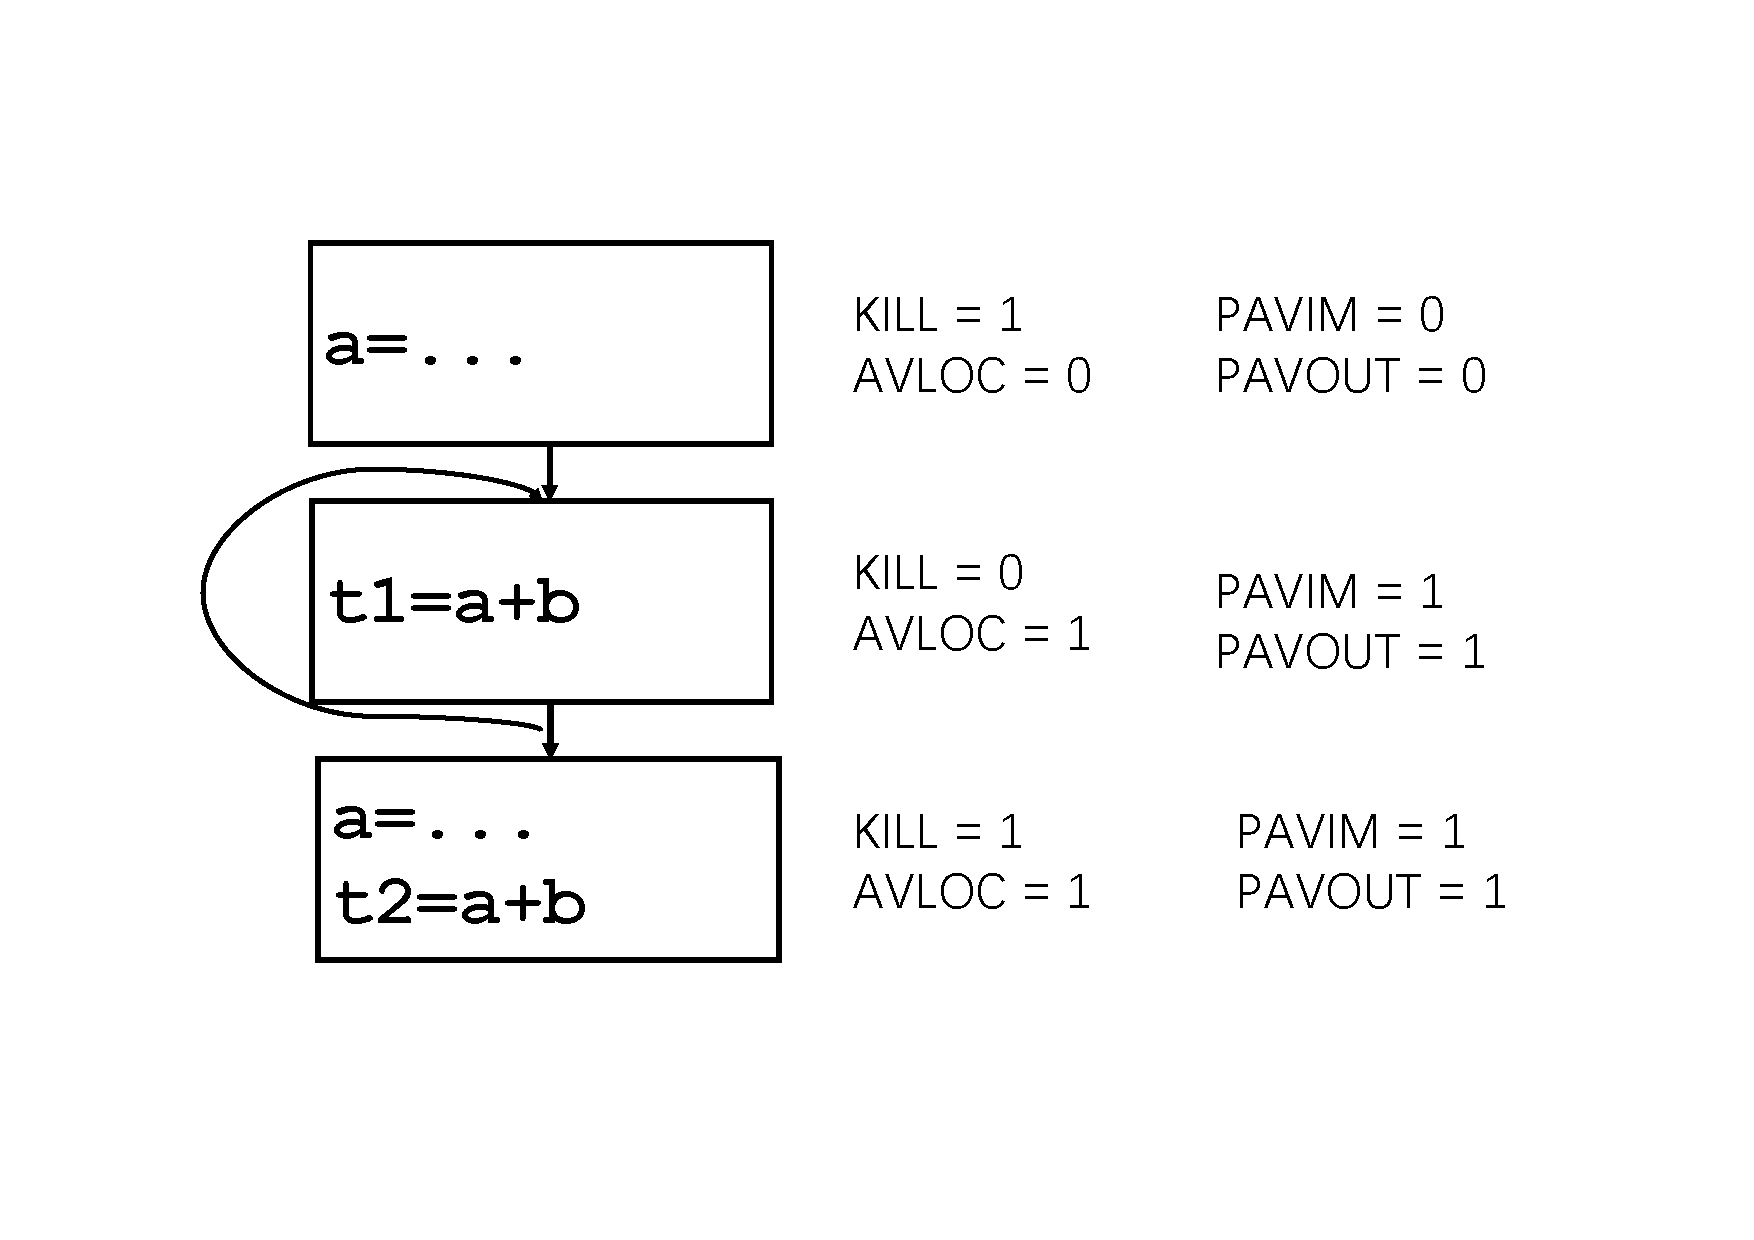
\includegraphics[width=0.8\textwidth]{p85.pdf}
         \caption{For \texttt{a+b}, the result Partially Available Expressions of dataflow analysis.}
         \label{fig:p85}
\end{figure}

\subsection{Finding Anticipated Expression}

For PRE, care must be taken that the hoisting would do no harm: Never introduce
 a new expression along any path. Otherwise the
hoisting will lengthen at least one trace of the program, defying optimality; even
worse, if the hoisted instruction throws an exception, the program’s semantics
change.



\begin{definition}{Local Anticipability(ANTLOC)}
An expression may
be locally anticipated in a block i if there is at least one
computation of the expression in the block i, and if the
commands appearing in the block before the first computation 
of the expression do not modify its operands. 
\end{definition}


\begin{center}
    \begin{tabular}{|c|c|}
   \hline Direction & backward\\
   \hline Meet operator & \( \cap \)\\
   \hline Lattice & \( \{ 0,1 \} \)\\
   \hline Top(T) & \( 1 \)\\
   \hline Boundary condition for exit node & \( 0 \) \\  
   \hline Initialization for internal nodes & \(\mathrm{T}\) \\
   \hline Finited escending chain? &\checkmark  \\
   \hline Transferfunction  &  \( ANTIN[i] = ANTLOC[i] \cup (ANTOUT[i] - KILL[i])\)\\
   \hline Monotone\&Distributive?  & \checkmark \\
   \hline ANTLOC & Expression is locally {\color{blue}anticipated(ANTLOC))} is upward exposed.\\
   \hline
   \end{tabular}  
   \end{center}

   \begin{figure}[H]
    \centering
     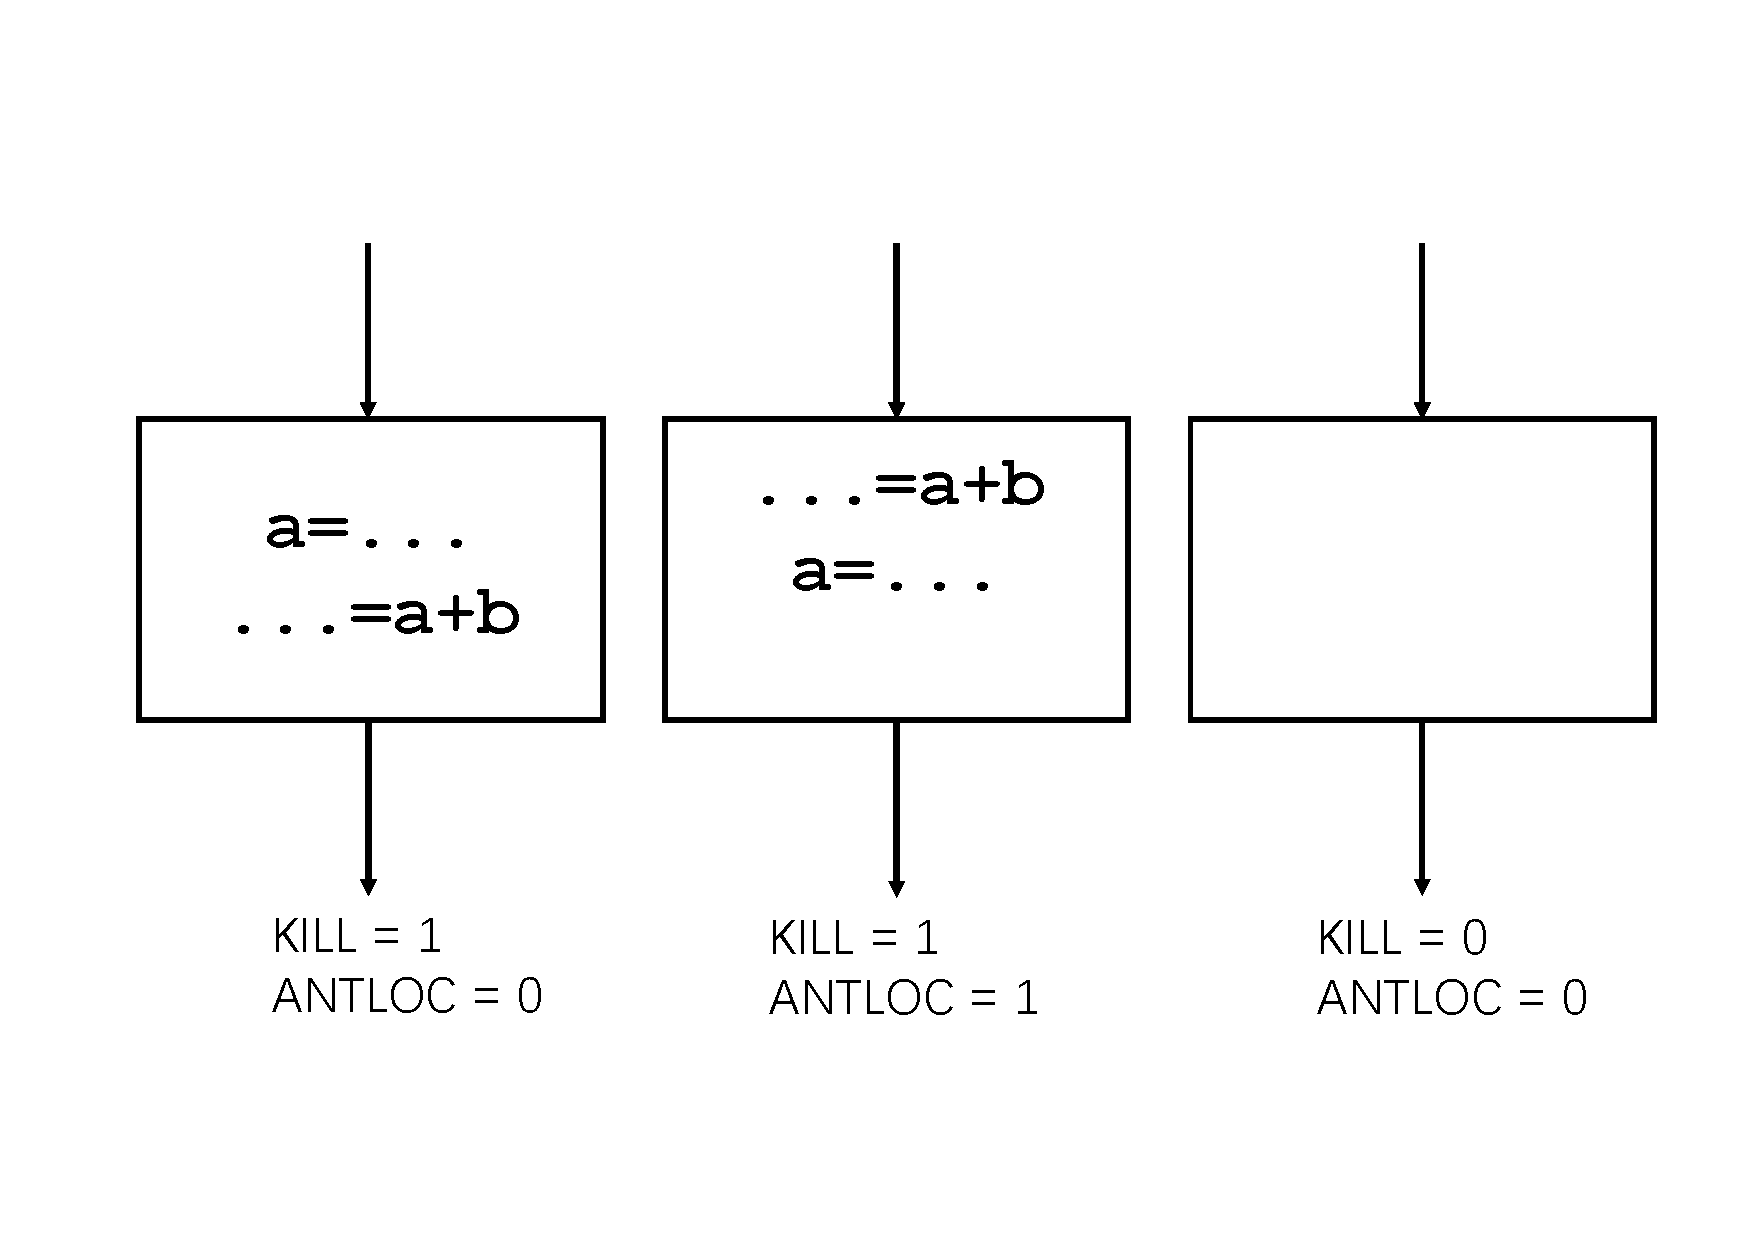
\includegraphics[width=0.8\textwidth]{p86.pdf}
         \caption{For \texttt{a+b}, the result of Anticipated Expression's transfer function within a basic block.}
         \label{fig:p86}
\end{figure}



\begin{figure}[H]
    \centering
     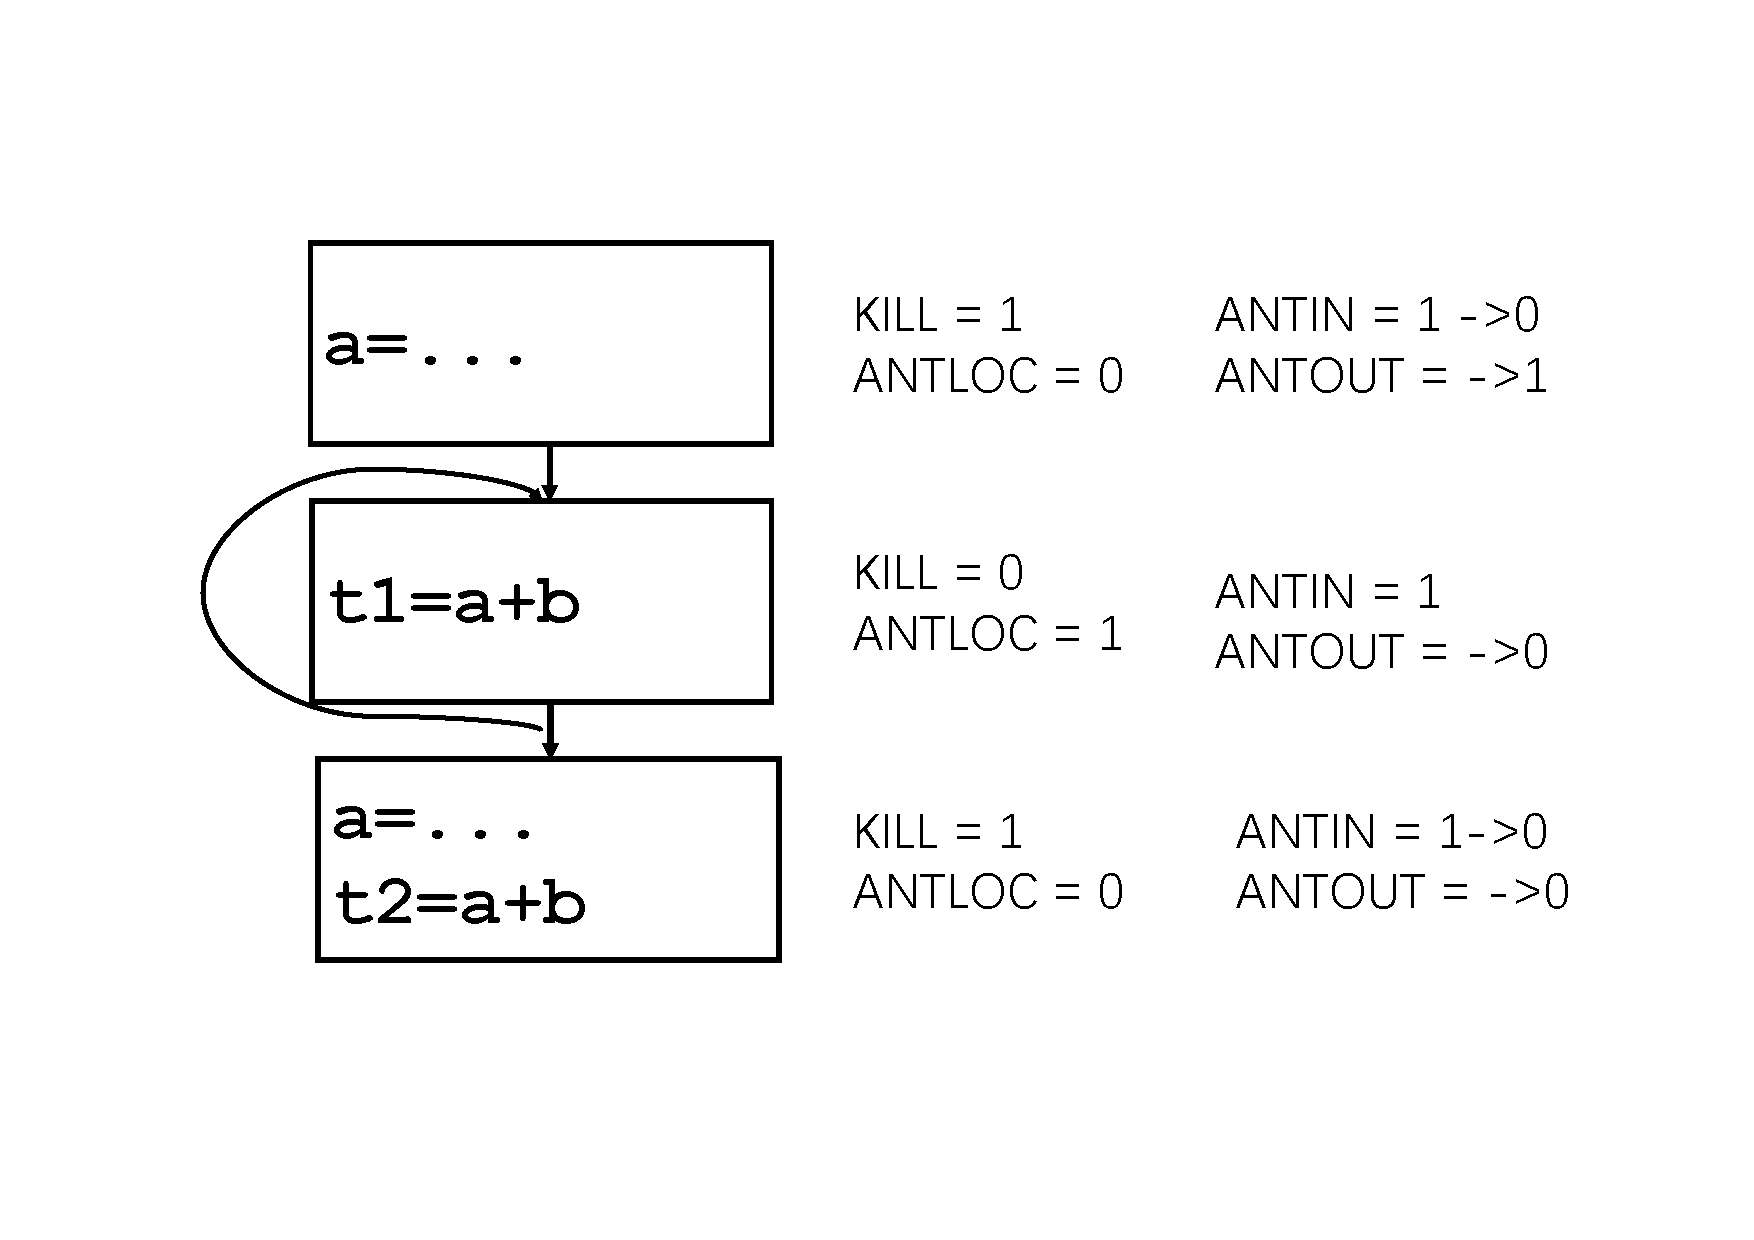
\includegraphics[width=0.8\textwidth]{p87.pdf}
         \caption{For \texttt{a+b}, the result Anticipated Expression of dataflow analysis.}
         \label{fig:p87}
\end{figure}


\subsection{Where Do we Want to Insert Computations?}


\begin{figure}[H]
    \centering
     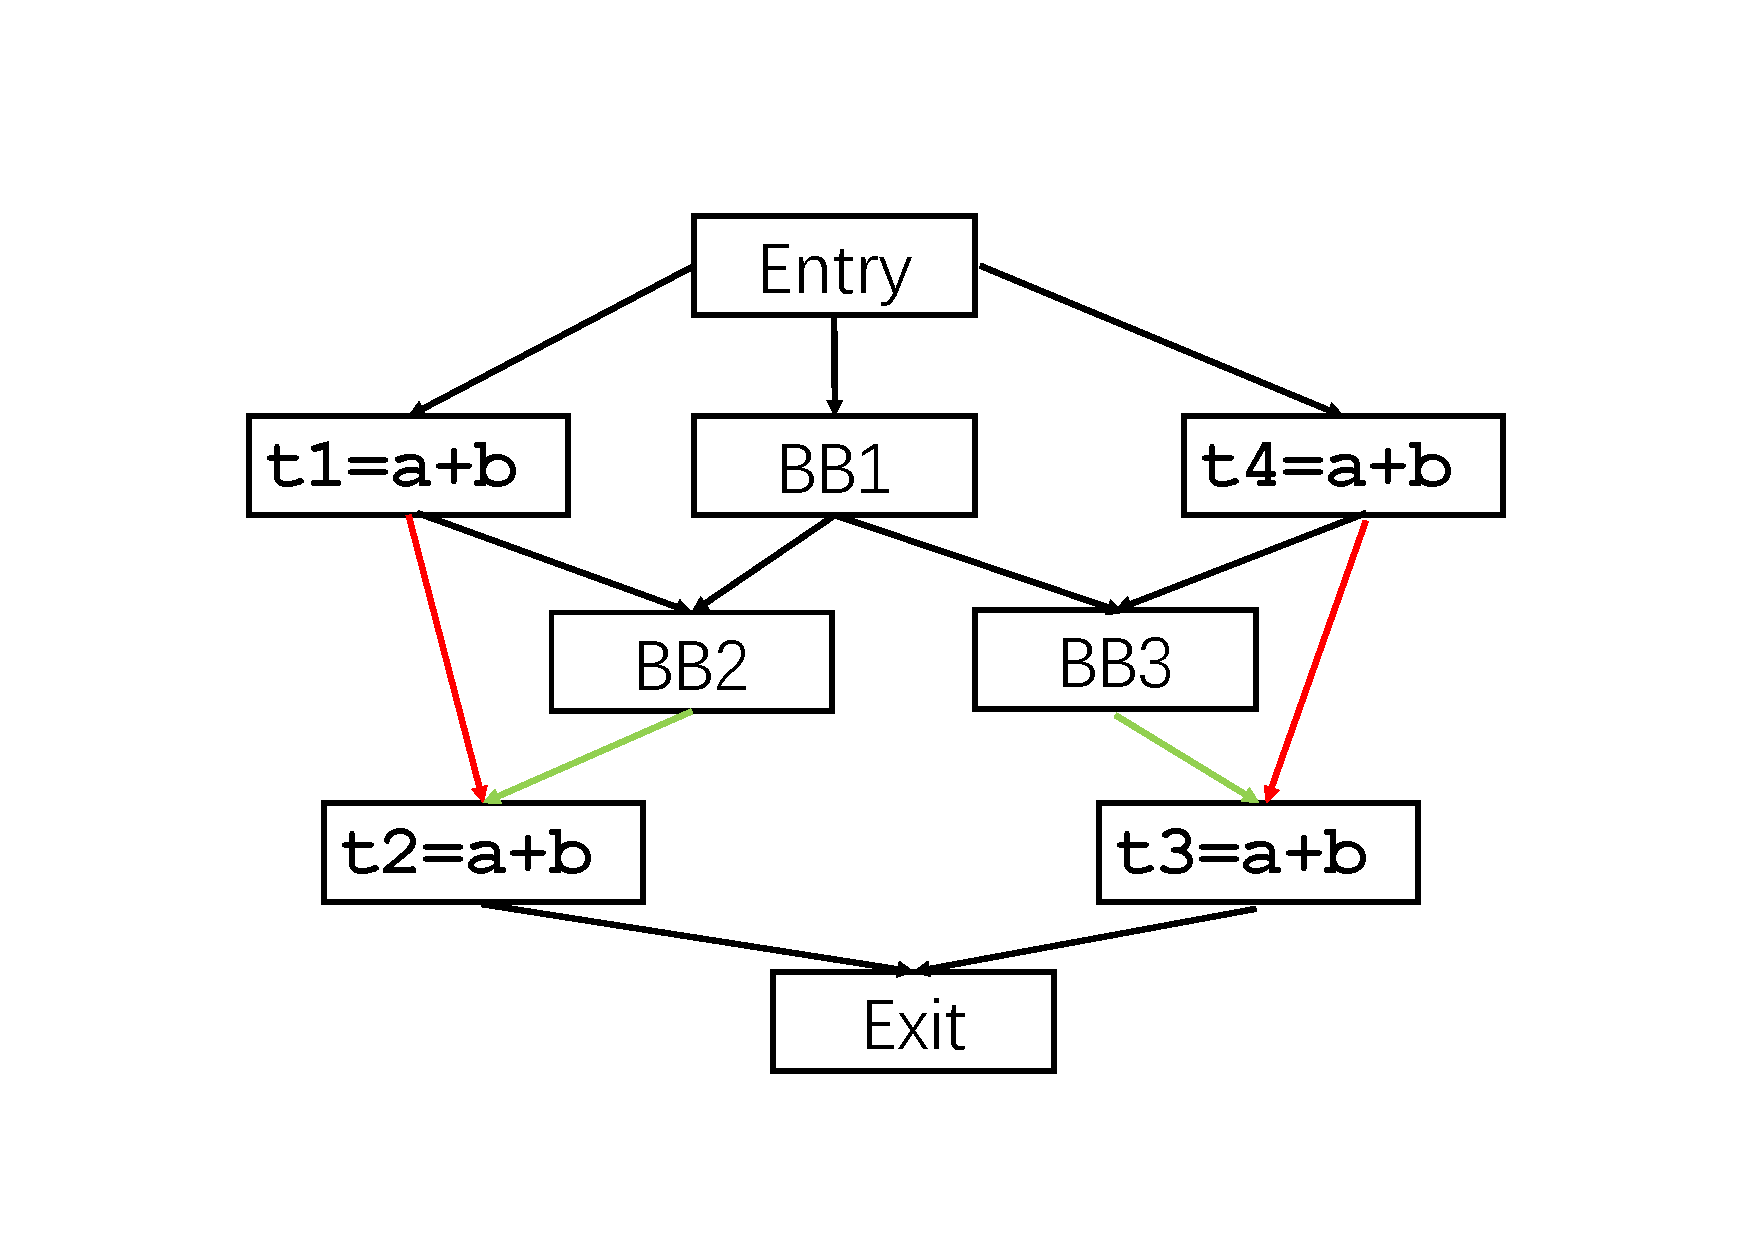
\includegraphics[width=0.8\textwidth]{p88.pdf}
         \caption{For \texttt{a+b}, \texttt{t2 = a + b} and \texttt{t3 = a + 4} are both partially redundant. But where can we insert the new computation \texttt{a + b} in order to optimally eliminate redundancy?
         The best choice is BB1 because this wil  make \texttt{a + b} fully redundant. But if we insert to BB2 and BB3, there are some path that calculate \texttt{a + b} more than once (e.g. Entry$\rightarrow$\texttt{t1= a+b} $\rightarrow$ BB2$\rightarrow$\texttt{t2= a+b}) }
         \label{fig:p88}
\end{figure}

We want to insert the new computation where it is not partially available there.


The key to partial redundancy
elimination is deciding where to add
computations of an expression to
change partial redundancies into full
redundancies (which may then be
optimized away).

We’ll start with an “enabling term.”

\[
    \mathrm{CONST}[i] = \mathrm{ANTIN}[i] \cap ( \mathrm{PAVIN}[i] \cup ( \neg \mathrm{KILL}[i] \cap \neg \mathrm{ANTLOC[i]}  ))
\]


This term say that we require the
expression to be:

\begin{itemize}
    \item  Anticipated at the start of block i (somebody wants the expression) \\
    {\huge and} 
    
        \item {\huge (2a)} The expression must be partially
        available (to perhaps transform
        into full availability)\\
        {\huge or} 
        \item {\huge (2b)} The block neither kills nor
        computes the expression.
   
\end{itemize}